\documentclass[11pt]{article}

% ----------------------------------------------------------------------------
%  TenaOS Technical Report — designed / distributable build
%  Compile with: pdflatex (run twice for TOC + bookmarks)
% ----------------------------------------------------------------------------

\usepackage[a4paper,margin=2.3cm,top=2.5cm,bottom=2.4cm]{geometry}
\usepackage[T1]{fontenc}
\usepackage[utf8]{inputenc}
\usepackage{charter}                 % clean, readable serif body
\usepackage[scaled=0.95]{helvet}     % Helvetica for headings (sans)
\usepackage{microtype}
\usepackage{booktabs}
\usepackage{array}
\usepackage{colortbl}
\usepackage{longtable}
\usepackage{enumitem}
\usepackage{etoolbox}
\usepackage{xcolor}
\usepackage{amssymb}
\usepackage{graphicx}
\usepackage{titlesec}
\usepackage{fancyhdr}
\usepackage{tikz}
\usepackage[most]{tcolorbox}
\usepackage{needspace}
\usepackage{ragged2e}
\usepackage{hyperref}
\usetikzlibrary{arrows.meta, positioning, fit, calc}

% ---------------- palette (inner pages only) ----------------
\definecolor{brandink}{HTML}{142033}
\definecolor{brandblue}{HTML}{14B8A6}
\definecolor{brandblued}{HTML}{14B8A6}
\definecolor{brandteal}{HTML}{14B8A6}
\definecolor{brandpurple}{HTML}{14B8A6}
\definecolor{brandwarm}{HTML}{14B8A6}
\definecolor{panebg}{HTML}{F5F8FC}
\definecolor{panebd}{HTML}{D7E1F0}
\definecolor{softgray}{HTML}{5A6B86}
\definecolor{rowalt}{HTML}{EFF4FB}
\definecolor{codebg}{HTML}{EEF2F8}
\definecolor{codeink}{HTML}{A14A06}

\hypersetup{
  colorlinks=true, linkcolor=brandblue, urlcolor=brandblue, citecolor=brandblue,
  pdftitle={TenaOS Technical Report},
  pdfauthor={Bezawit Alemu, Brook Ayalneh},
  pdfsubject={Local-first clinical AI operating system},
  bookmarksnumbered=true, bookmarksopen=true
}

% ---------------- shortcuts ----------------
\newcommand{\Product}{TenaOS}
\newcommand{\Gemma}{Gemma 4 E4B}
\newcommand{\OpenMRS}{OpenMRS}
\newcommand{\CIEL}{CIEL}
\newcommand{\WHO}{WHO/MSF}
\newcommand{\code}[1]{{\setlength{\fboxsep}{1.7pt}\colorbox{codebg}{\textcolor{codeink}{\small\ttfamily #1}}}}

\setlist[itemize]{leftmargin=1.4em, itemsep=3pt, topsep=4pt, parsep=0pt}
\setlist[enumerate]{leftmargin=1.6em, itemsep=4pt, topsep=4pt, parsep=0pt}
\renewcommand{\arraystretch}{1.3}
\setlength{\parindent}{0pt}
\setlength{\parskip}{0.7em}
\linespread{1.07}
\setlength{\emergencystretch}{3em}
\color{brandink}

% ---------------- page-break discipline ----------------
\widowpenalty=10000          % no single line stranded at top of page
\clubpenalty=10000           % no single line stranded at bottom of page
\displaywidowpenalty=10000
\brokenpenalty=10000
\interlinepenalty=200
\raggedbottom                % consistent bottoms instead of stretched glue

% never leave a heading stranded at the foot of a page: require space for the
% heading plus the first few lines of its body, else push to the next page.
\pretocmd{\section}{\Needspace*{7\baselineskip}}{}{}
\pretocmd{\subsection}{\Needspace*{7\baselineskip}}{}{}

% ---------------- section styling ----------------
\titleformat{\section}
  {\sffamily\Large\bfseries\color{brandink}}
  {\colorbox{brandblue}{\makebox[1.55em][c]{\textcolor{white}{\thesection}}}\hspace{0.65em}}
  {0pt}{}[{\vspace{3pt}\color{panebd}\titlerule[1.1pt]}]
\titlespacing*{\section}{0pt}{2.0em}{1.0em}

\titleformat{\subsection}
  {\sffamily\large\bfseries\color{brandblued}}
  {\textcolor{brandteal}{\rule[0.45ex]{0.55em}{0.55em}}\hspace{0.55em}}
  {0pt}{}
\titlespacing*{\subsection}{0pt}{1.5em}{0.5em}

% ---------------- header / footer ----------------
\pagestyle{fancy}
\fancyhf{}
\renewcommand{\headrulewidth}{0pt}
\renewcommand{\footrulewidth}{0pt}
\fancyhead[L]{\sffamily\footnotesize\color{softgray}\strut\textbf{\textcolor{brandblue}{Tena}OS}\ \,Technical Report}
\fancyhead[R]{\sffamily\footnotesize\color{softgray}\strut AI-Native Clinical Operating System}
\fancyfoot[R]{\sffamily\footnotesize\color{softgray}\thepage}

% ---------------- reusable boxes ----------------
\newtcolorbox{abstractbox}{
  enhanced, colback=panebg, colframe=brandblue, boxrule=0pt,
  leftrule=3.5pt, arc=2pt, left=15pt, right=15pt, top=12pt, bottom=12pt
}
\newtcolorbox{safetybox}{
  enhanced, colback=brandwarm!7, colframe=brandwarm, boxrule=0pt,
  leftrule=3.5pt, arc=2pt, left=13pt, right=13pt, top=10pt, bottom=10pt
}
\newtcolorbox{infobox}{
  enhanced, colback=brandteal!7, colframe=brandteal, boxrule=0pt,
  leftrule=3.5pt, arc=2pt, left=13pt, right=13pt, top=10pt, bottom=10pt
}

% stat card command: \statcard{value}{label}
\newcommand{\statcard}[2]{%
  \begin{tcolorbox}[enhanced, colback=white, colframe=panebd, boxrule=0.8pt,
    arc=3pt, left=9pt, right=9pt, top=9pt, bottom=9pt, height=2.7cm, valign=center]
    \RaggedRight
    {\sffamily\fontsize{19}{21}\selectfont\bfseries\color{brandblue} #1}\\[3pt]
    {\sffamily\footnotesize\color{softgray} #2}
  \end{tcolorbox}}

% labeled pill for tables
\newcommand{\pill}[2]{{\sffamily\setlength{\fboxsep}{2.4pt}\colorbox{#1!15}{\textcolor{#1}{\scriptsize\bfseries #2}}}}

% diagram frame with auto-fit-to-width content
\newtcolorbox{diagrambox}[1]{
  enhanced, colback=white, colframe=panebd, boxrule=0.8pt, arc=3pt,
  left=8pt, right=8pt, top=22pt, bottom=14pt,
  overlay={\node[anchor=north west, font=\sffamily\footnotesize\bfseries\color{softgray}]
    at ([xshift=11pt,yshift=-7pt]frame.north west) {\textcolor{brandteal}{\footnotesize$\blacktriangleright$}\ #1};
    \draw[panebd] ([yshift=-18pt]frame.north west) -- ([yshift=-18pt]frame.north east);}
}
% \diagramfig{title}{tikzpicture} — scales down only if wider than the column
\newcommand{\diagramfig}[2]{%
  \par\vspace{0.4em}
  \Needspace*{11\baselineskip}%
  \begin{diagrambox}{#1}
  \centering
  \resizebox{\ifdim\width>\linewidth\linewidth\else\width\fi}{!}{#2}\par
  \end{diagrambox}
  \vspace{0.4em}\par}

% tikz node styles
\tikzset{
  fbox/.style={draw=panebd, fill=panebg, rounded corners=3pt, align=center,
    minimum height=0.9cm, minimum width=2.0cm, font=\sffamily\footnotesize, text=brandink, line width=0.7pt},
  abox/.style={draw=brandblue, fill=brandblue!10, rounded corners=3pt, align=center,
    minimum height=0.9cm, minimum width=2.0cm, font=\sffamily\footnotesize\bfseries, text=brandblued, line width=0.9pt},
  flow/.style={-{Latex[length=2.4mm]}, draw=softgray, line width=0.8pt}
}

\begin{document}

% ============================================================ COVER (minimal, no color, no graphics)
\begin{titlepage}
\thispagestyle{empty}
\color{black}
\centering
\vspace*{0.30\textheight}

{\fontsize{60}{64}\selectfont\bfseries\color{brandteal} TenaOS\par}
\vspace{14pt}
{\Large Technical Report\par}

\vfill

{\large 2026\par}
\vspace{12pt}
{\large by Bezawit Alemu, Brook Ayalneh\par}
\vspace*{0.12\textheight}
\end{titlepage}
\color{brandink}

% ============================================================ ABSTRACT
\section{Abstract}

\begin{abstractbox}
\Product{} is a local-first clinical AI operating system that lets health facilities build and operate standards-based digital health workflows through natural language. It combines \OpenMRS{}, \Gemma{}, a \WHO{} guideline knowledge base, a \CIEL{} terminology knowledge base, deterministic middleware, and a mandatory clinician review layer, inside a locally deployable stack.

\smallskip
The problem \Product{} addresses is \textbf{implementation, not technology}. The open foundations of digital health already exist. \OpenMRS{}, \CIEL{}, and published WHO and MSF guidance are open, proven, and freely available, yet they stay locked behind a team of specialists for customization, configuration, and maintenance that low-resource clinics cannot sustain.

\smallskip
Every conventional rollout assumes a software team, a network connection, and weeks of form building, terminology mapping, and reporting design; when the grant ends and the specialists leave, the clinic returns to paper. \Product{} removes that implementation tax. It turns the work of an informatics team into a local, auditable, clinician-reviewed conversation, so the people who actually run the clinic can build and operate standards-based digital health themselves.

\smallskip
The system runs as a single local container with \OpenMRS{}, MariaDB, Qdrant, \Gemma{} served through \code{llama.cpp}, and the TenaAgent orchestration service. The model never writes directly to \OpenMRS{}. It operates through allow-listed tools and structured draft stores; final writes go through deterministic validation and clinician approval.
\end{abstractbox}

% ============================================================ CONTRIBUTIONS
\section{Contributions}

\Product{} makes four technical contributions.

\begin{enumerate}
  \item \textbf{A local-first clinical AI runtime.} \Product{} integrates \OpenMRS{}, \Gemma{}, local guideline retrieval, local terminology retrieval, and TenaAgent into a single deployable stack.
  \item \textbf{Two complementary local knowledge bases.} The \WHO{} knowledge base grounds recommendations and patient materials in guideline evidence; the \CIEL{} knowledge base resolves natural language to standards-based \OpenMRS{} concepts.
  \item \textbf{A constrained clinical agent pattern.} \Gemma{} interacts through allow-listed tools, retrieval services, draft stores, deterministic validators, and \OpenMRS{} writers instead of uncontrolled free-text actions. The architecture treats the model as a planner and proposer, while concept validation, schema construction, query compilation, and persistence stay deterministic.
  \item \textbf{A GEPA-then-LoRA adaptation path.} \Product{} first optimizes prompts against the real production pipeline with GEPA, then distils the validated traces into a single task-tagged LoRA adapter, merged into the model weights at deployment. A single multi-task adapter, routed by task tags such as \code{[form]}, \code{[report]}, \code{[scribe]}, and \code{[cds]}, serves every workflow without per-task model swaps.
\end{enumerate}

% ============================================================ REQUIREMENTS
\section{Design Requirements}

\Product{} targets clinics that cannot assume continuous internet, cloud inference, or a local implementation team. The system is built around these requirements:

\begin{itemize}
  \item \textbf{Local ownership:} patient data and model inference stay on facility-owned infrastructure.
  \item \textbf{Standards compatibility:} \OpenMRS{} remains the record system; \CIEL{} and FHIR-style query plans preserve interoperability.
  \item \textbf{Clinical review:} every AI-generated clinical artifact remains reviewable and editable by a clinician.
  \item \textbf{Deterministic trust boundary:} middleware validates concept IDs, datatypes, retired status, schema structure, reporting plans, and \OpenMRS{} writes.
  \item \textbf{Evidence grounding:} CDS and patient education search local \WHO{} evidence rather than answering from model memory.
  \item \textbf{Auditability:} tool calls, retrieval steps, drafts, and final outputs are persisted or streamed as traces.
\end{itemize}

% ============================================================ OVERVIEW
\section{System Overview}

At a high level, \Product{} converts natural clinical language into standards-based clinical artifacts.

\diagramfig{High-level safety invariant}{%
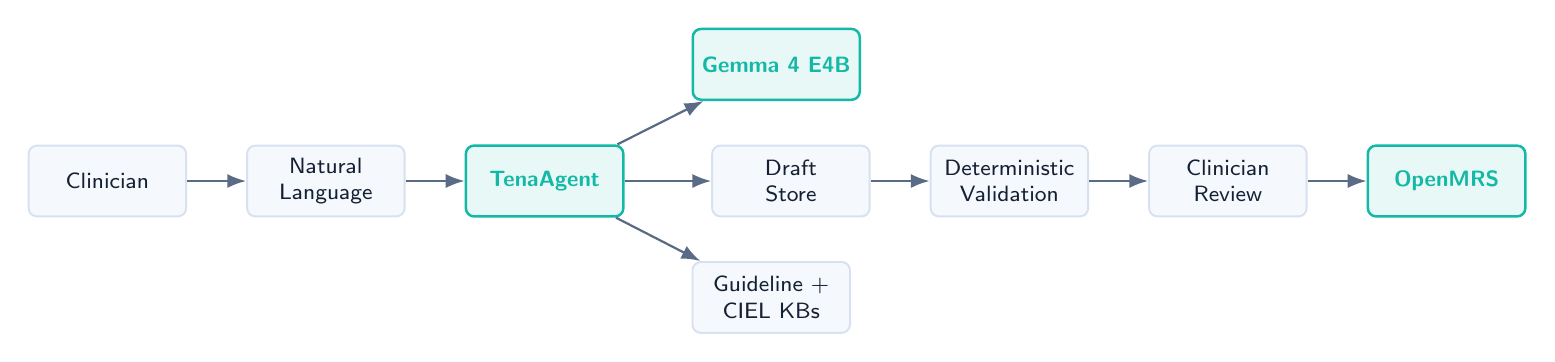
\begin{tikzpicture}[node distance=0.6cm and 0.75cm]
\node[fbox] (clin) {Clinician};
\node[fbox, right=of clin] (input) {Natural\\Language};
\node[abox, right=of input] (agent) {TenaAgent};
\node[abox, above right=0.55cm and 0.85cm of agent] (gemma) {Gemma 4 E4B};
\node[fbox, right=1.1cm of agent] (draft) {Draft\\Store};
\node[fbox, below right=0.55cm and 0.85cm of agent] (kb) {Guideline +\\CIEL KBs};
\node[fbox, right=of draft] (val) {Deterministic\\Validation};
\node[fbox, right=of val] (rev) {Clinician\\Review};
\node[abox, right=of rev] (omrs) {OpenMRS};
\draw[flow] (clin)--(input); \draw[flow] (input)--(agent);
\draw[flow] (agent)--(gemma); \draw[flow] (agent)--(kb); \draw[flow] (agent)--(draft);
\draw[flow] (draft)--(val); \draw[flow] (val)--(rev); \draw[flow] (rev)--(omrs);
\end{tikzpicture}}

The deployed runtime is a single-container stack. nginx is the only public ingress. TenaAgent, \OpenMRS{}, Qdrant, Gemma, and both KB daemons communicate on container-local ports.

\diagramfig{Single-container deployment topology}{%
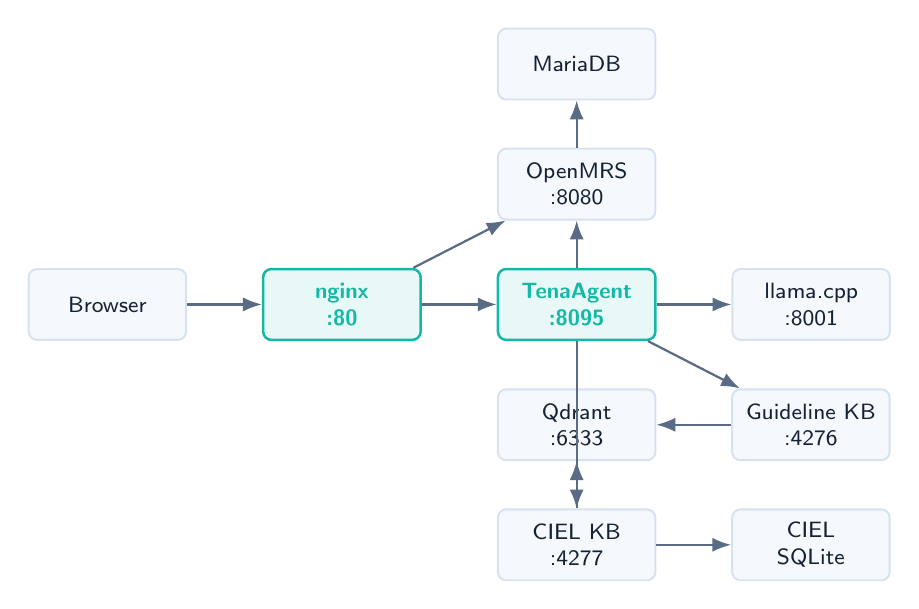
\begin{tikzpicture}[node distance=0.6cm and 0.95cm]
\node[fbox] (browser) {Browser};
\node[abox, right=of browser] (nginx) {nginx\\:80};
\node[abox, right=of nginx] (agent) {TenaAgent\\:8095};
\node[fbox, above=of agent] (openmrs) {OpenMRS\\:8080};
\node[fbox, above=of openmrs] (mariadb) {MariaDB};
\node[fbox, right=of agent] (llama) {llama.cpp\\:8001};
\node[fbox, below=of agent] (qdrant) {Qdrant\\:6333};
\node[fbox, right=of qdrant] (guideline) {Guideline KB\\:4276};
\node[fbox, below=of qdrant] (ciel) {CIEL KB\\:4277};
\node[fbox, right=of ciel] (sqlite) {CIEL\\SQLite};
\draw[flow] (browser)--(nginx); \draw[flow] (nginx)--(agent); \draw[flow] (nginx)--(openmrs);
\draw[flow] (agent)--(llama); \draw[flow] (agent)--(guideline); \draw[flow] (agent)--(ciel);
\draw[flow] (agent)--(openmrs); \draw[flow] (guideline)--(qdrant); \draw[flow] (ciel)--(qdrant);
\draw[flow] (ciel)--(sqlite); \draw[flow] (openmrs)--(mariadb);
\end{tikzpicture}}

The main source-backed components are:
\begin{itemize}
  \item \code{TenaOS-Frontend/}: React clinical workspace.
  \item \code{TenaOS-Backend/}: \OpenMRS{} Reference Application 3 packaging and metadata contracts.
  \item \code{TenaAgent/}: Python orchestration service for all LLM-mediated workflows.
  \item \code{TenaOS-LLM/}: \code{llama.cpp} serving layout for \Gemma{} GGUF, the multimodal projector, and the merged task-tagged \Product{} LoRA adapter.
  \item \code{TenaOS-KnowledgeBase/}: Qdrant-backed retrieval daemon for \WHO{} guidelines and \CIEL{} semantic search.
  \item \code{TenaOS-CIEL/}: \CIEL{} SQLite, FTS5 search, bundle expansion, and Qdrant indexing code.
  \item \code{scripts/fetch-models.sh}: artifact bootstrap for Gemma, EmbedGemma, CIEL SQLite, Qdrant snapshots, and SapBERT.
  \item \code{docker/restore-qdrant.sh}: supervised restore of the guideline and CIEL snapshots.
\end{itemize}

\textbf{Deployment tiers.} The same stack ships in two hardware profiles from one image. An \emph{edge-server tier} (mini-PC, 16--32\,GB RAM, optional small GPU) serves \Gemma{} at BF16 with the LoRA adapter weights merged for full-fidelity inference. A \emph{tablet tier} (consumer Android / ARM device) serves a \code{Q4\_K\_M} quantization of the same weights with the merged adapter, trading a small quality margin for a footprint that runs without a server. Model inference, \OpenMRS{}, \CIEL{}, and Qdrant remain fully local in both tiers.

% ============================================================ KNOWLEDGE
\Needspace*{20\baselineskip}
\section{Knowledge Systems}

\Product{} has two local knowledge systems because clinical evidence and clinical terminology serve different roles.

\begin{infobox}
\textbf{WHO/MSF Guideline KB} answers: \emph{``What does the evidence or protocol say?''} It supports CDS, patient education, and form design.

\smallskip
\textbf{CIEL Terminology KB} answers: \emph{``Which standard concept should represent this clinical idea in OpenMRS?''} It supports forms, scribing, reports, and safe persistence.
\end{infobox}

\subsection{WHO/MSF Guideline Knowledge Base}

\textbf{Source and extraction.} The \WHO{} KB is composed of WHO and MSF clinical guidance documents, including clinical practice guidelines, pocket guides, technical reports, rapid advice, consolidated guidance, and MSF protocol-style material. The offline build runs in the \code{kb-pipeline} build tree; it is a one-time, build-time process and is not part of the clinic runtime.

PDFs are processed through an OCR and normalization pipeline that converts each document into structured, page-aware JSON, preserving text, heading hierarchy, footnotes, and confidence metadata. The pipeline operates against a \textbf{19,900-page} extraction budget. The current build tree contains \textbf{401 chunk JSONL files} and \textbf{69,476 guideline chunks}.

\diagramfig{Guideline KB build pipeline}{%

\begin{tikzpicture}[node distance=0.6cm and 0.6cm]
\node[fbox] (pdf) {WHO/MSF\\PDFs};
\node[fbox, right=of pdf] (pulse) {OCR /\\Normalize};
\node[fbox, right=of pulse] (docling) {Docling\\JSON};
\node[fbox, right=of docling] (chunk) {Chunk +\\Enrich};
\node[fbox, right=of chunk] (embed) {EmbedGemma\\+ BM25};
\node[abox, right=of embed] (qdrant) {Qdrant\\Snapshot};
\draw[flow] (pdf)--(pulse); \draw[flow] (pulse)--(docling); \draw[flow] (docling)--(chunk);
\draw[flow] (chunk)--(embed); \draw[flow] (embed)--(qdrant);
\end{tikzpicture}}

\textbf{Normalization and chunking.} The pipeline converts cleaned markdown into Docling JSON, classifies documents, fixes heading levels, chunks documents, enriches metadata, post-processes chunks, and backfills metadata. Shared chunking logic identifies recommendation signals such as ``WHO recommends,'' ``It is recommended that,'' ``Good practice statement,'' and GRADE certainty symbols, classifying content into \code{recommendation}, \code{implementation}, \code{etd}, \code{methods\_pico}, \code{background}, \code{research\_gap}, \code{annex}, and \code{scope}. Each chunk stores heading paths, provenance, source URL, document type, disease area, content hash, version date, token count, recommendation number, and retrieval priority. Superseded chunks can be hard-dropped with priority \code{0.0}.

\textbf{Embedding and indexing.} \code{embed\_chunks\_gpu.py} embeds contextualized chunks with EmbedGemma 300M (heading path plus body, dimension 768). Long chunks are split into up to three 10,000-character windows, embedded independently, mean-pooled, and normalized. \code{build\_qdrant.py} aligns chunk IDs with embeddings, cleans OCR artifacts, filters duplicates, computes BM25 sparse vectors, and writes Qdrant points with dense vector \code{embedgemma}, sparse vector \code{bm25}, payload indexes, and stable UUID5 IDs. The resulting \code{who\_msf\_guidelines.snapshot} is about \textbf{448.8 MB}.

\textbf{Runtime retrieval.} The daemon in \code{kb\_guidelines/daemon.py} exposes \code{/health}, \code{/stats}, and \code{/search}, binds locally by default, and can require an \code{X-TenaOS-KB-Secret} shared secret. Search modes are \code{lex} (BM25 sparse), \code{sem} (EmbedGemma dense), and \code{rrf} (reciprocal-rank fusion). The reranker performs corruption filtering, synonym expansion, action-query detection, content-type boosts, actionability boosts for dose/route/frequency text, domain coherence penalties, source diversity penalties, condition/title exclusions, population/intent reranking, and low-confidence flags.

\subsection{CIEL Terminology Knowledge Base}

\textbf{Source and SQLite build.} \CIEL{} is the terminology layer that makes \Product{} interoperable with \OpenMRS{}. The local SQLite store is built from an OpenConceptLab CIEL export; the checked local artifact is CIEL \code{v2026-03-23}. \code{ciel\_search/pipeline.py} streams the export with \code{ijson} and writes \code{source\_metadata}, \code{concept\_bundles}, \code{concept\_mappings}, and a \code{concept\_search\_fts} FTS5 index. The resulting store holds \textbf{58,687 concepts} (of which \textbf{3,205} are retired), \textbf{298,905 concept mappings}, \textbf{8,545 question-and-answer edges}, and \textbf{3,259 concept-set edges}; all \textbf{58,687 concepts} are hydrated into bundles.

Each concept bundle preserves the raw concept JSON and stores UUID, display name, class, datatype, retired status, locales, names, descriptions, answers, set members, external mappings, incoming relationships, source version, and generated search text.

\diagramfig{CIEL build and runtime hydration}{%
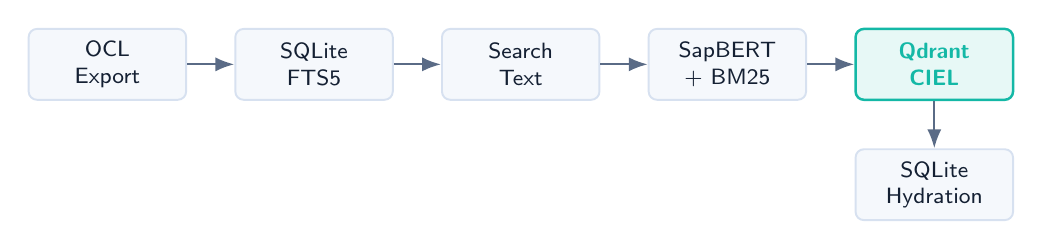
\begin{tikzpicture}[node distance=0.6cm and 0.6cm]
\node[fbox] (ocl) {OCL\\Export};
\node[fbox, right=of ocl] (sqlite) {SQLite\\FTS5};
\node[fbox, right=of sqlite] (text) {Search\\Text};
\node[fbox, right=of text] (vectors) {SapBERT\\+ BM25};
\node[abox, right=of vectors] (qdrant) {Qdrant\\CIEL};
\node[fbox, below=of qdrant] (hydrate) {SQLite\\Hydration};
\draw[flow] (ocl)--(sqlite); \draw[flow] (sqlite)--(text); \draw[flow] (text)--(vectors);
\draw[flow] (vectors)--(qdrant); \draw[flow] (qdrant)--(hydrate);
\end{tikzpicture}}

\textbf{Search text and bundle expansion.} Search text is built from preferred names, synonyms, descriptions, answer labels, set-member labels, external source codes, and relationship labels --- because a query like ``BP,'' ``blood pressure,'' or ``systolic'' must still recover usable \OpenMRS{} concepts. SQLite remains the authority for deterministic lookups and bundle expansion, supporting exact search, FTS5 fallback, Q-and-A answer expansion, concept-set member expansion, and form-ready seed discovery.

\textbf{Semantic index.} The semantic index uses SapBERT (\code{cambridgeltl/SapBERT-from-PubMedBERT-fulltext}) for dense concept embeddings and the shared BM25 encoder for sparse vectors. The Qdrant collection \code{ciel\_concepts} stores dense vector \code{sapbert}, sparse vector \code{bm25}, and payload fields for concept identity. The local \code{ciel\_concepts.snapshot} is about \textbf{326.3 MB}.

\textbf{Runtime resolution.} Discovery is hybrid: Qdrant returns candidate concept IDs via SapBERT + BM25 RRF, then SQLite hydrates them through \code{CielSearchService}. The runtime never trusts vector search alone; final decisions use class, datatype, retired status, duplicate checks, answer availability, set membership, and \OpenMRS{} UUID compatibility.

% ============================================================ FEATURES
\section{Feature Architecture}

TenaOS exposes five clinician-facing workflows on the shared agent runtime --- the natural-language form builder, the SOAP scribe, clinical decision support, patient education, and plain-language reporting. Each one combines local retrieval, a constrained agent loop, deterministic checks, and a clinician review step before anything is persisted. The subsections below describe each workflow with its data flow.

\subsection{Natural-Language Form Builder}

The form builder is the most mature workflow and the primary GEPA optimization target. The production pipeline (\code{form\_pipeline/runner.py}):

\begin{enumerate}
  \item Research the request against the \WHO{} KB.
  \item Produce a structured question worklist.
  \item Resolve worklist items against \CIEL{}.
  \item Commit fields into a draft basket.
  \item Run a bounded coverage-repair pass.
  \item Build an \OpenMRS{} schema.
  \item Produce a deterministic summary for clinician review.
  \item Publish only after approval.
\end{enumerate}

\diagramfig{Form builder pipeline}{%
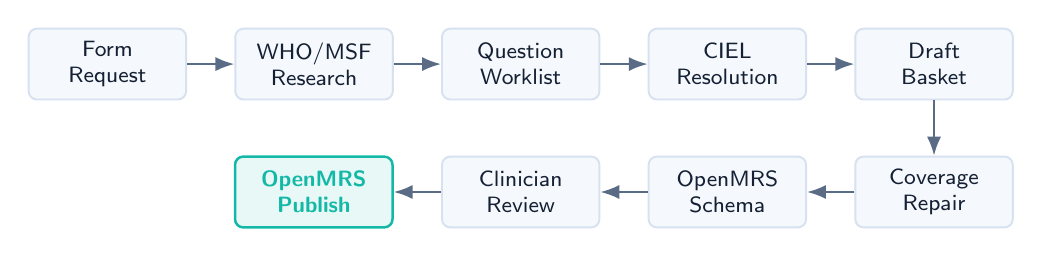
\begin{tikzpicture}[node distance=0.6cm and 0.6cm]
\node[fbox] (req) {Form\\Request};
\node[fbox, right=of req] (res) {WHO/MSF\\Research};
\node[fbox, right=of res] (work) {Question\\Worklist};
\node[fbox, right=of work] (ciel) {CIEL\\Resolution};
\node[fbox, right=of ciel] (basket) {Draft\\Basket};
\node[fbox, below=0.7cm of basket] (repair) {Coverage\\Repair};
\node[fbox, left=of repair] (schema) {OpenMRS\\Schema};
\node[fbox, left=of schema] (review) {Clinician\\Review};
\node[abox, left=of review] (pub) {OpenMRS\\Publish};
\draw[flow] (req)--(res); \draw[flow] (res)--(work); \draw[flow] (work)--(ciel);
\draw[flow] (ciel)--(basket); \draw[flow] (basket)--(repair); \draw[flow] (repair)--(schema);
\draw[flow] (schema)--(review); \draw[flow] (review)--(pub);
\end{tikzpicture}}

\OpenMRS{} form publication (\code{openmrs\_writer.py}) is a three-step REST operation: create Form metadata, upload the JSON schema as ClobData, and bind the schema as a form resource. If a later step fails, the created form is retired so only usable forms appear in the form list.

\subsection{SOAP Scribe}

The scribe accepts text, voice, or image. For voice input, the route accepts multipart audio, converts it to 16\,kHz mono WAV with \code{ffmpeg}, base64-encodes it, and sends it to Gemma using an audio content block; \Gemma{}'s native speech understanding transcribes \emph{English and Amharic} voice directly through the same inference pass, so no separate ASR engine is required. For image input (for example a photograph of a paper intake form, a handwritten note, or a lab slip), the route encodes the image through the multimodal projector and \Gemma{} reads it into the same SOAP extraction step. For Amharic notes, an optional translation step normalises the note to English before extraction to maximise CIEL resolution; native Amharic transcription and translation are handled by the model rather than an external pipeline.

\diagramfig{Scribe workflow}{%
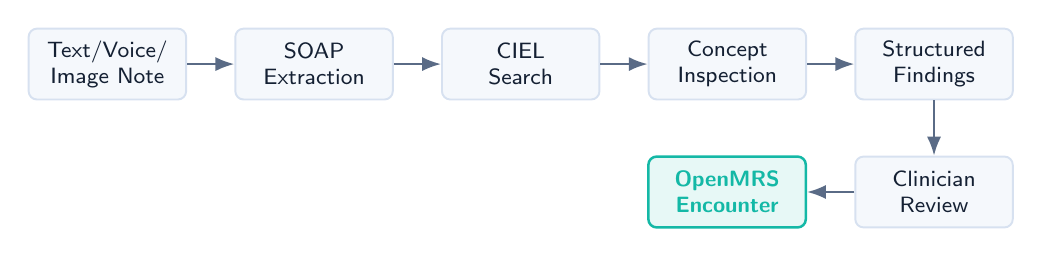
\begin{tikzpicture}[node distance=0.6cm and 0.6cm]
\node[fbox] (note) {Text/Voice/\\Image Note};
\node[fbox, right=of note] (soap) {SOAP\\Extraction};
\node[fbox, right=of soap] (search) {CIEL\\Search};
\node[fbox, right=of search] (inspect) {Concept\\Inspection};
\node[fbox, right=of inspect] (struct) {Structured\\Findings};
\node[fbox, below=0.7cm of struct] (review) {Clinician\\Review};
\node[abox, left=of review] (enc) {OpenMRS\\Encounter};
\draw[flow] (note)--(soap); \draw[flow] (soap)--(search); \draw[flow] (search)--(inspect);
\draw[flow] (inspect)--(struct); \draw[flow] (struct)--(review); \draw[flow] (review)--(enc);
\end{tikzpicture}}

The model extracts SOAP sections, coded concepts, observations, and medications. The backend validates and resolves CIEL IDs before review. Unresolved items are carried forward for clinician review rather than silently written.

\subsection{Clinical Decision Support}

Clinical decision support runs as an agentic ReAct loop --- \code{KbAgentLoop} in \code{tool\_loop.py}. When a clinician opens the AI-insight panel, the frontend calls \code{POST /insights/patient/\{uuid\}}; TenaAgent starts a background trace and streams progress to the browser over Server-Sent Events (\code{GET /insights/\{traceId\}/events}). First, \code{OpenMrsClient.build\_patient\_context} assembles a \code{PatientInsightContext} from OpenMRS REST reads --- demographics, active visit, conditions, allergies, drug orders, and recent observation snippets --- and \code{\_build\_patient\_summary} condenses it for Gemma.

\diagramfig{Clinical Decision Support --- agentic ReAct loop over the WHO/MSF KB}{%
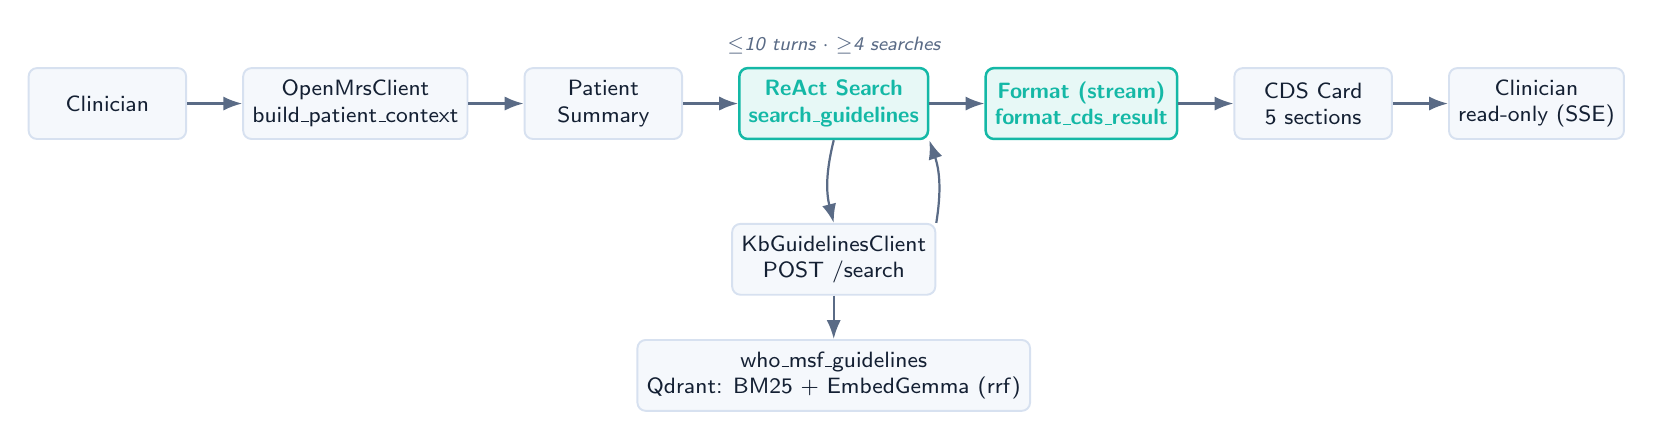
\begin{tikzpicture}[node distance=0.62cm and 0.7cm]
\node[fbox] (clin) {Clinician};
\node[fbox, right=of clin] (ctx) {OpenMrsClient\\build\_patient\_context};
\node[fbox, right=of ctx] (sum) {Patient\\Summary};
\node[abox, right=of sum] (search) {ReAct Search\\search\_guidelines};
\node[abox, right=of search] (fmt) {Format (stream)\\format\_cds\_result};
\node[fbox, right=of fmt] (card) {CDS Card\\5 sections};
\node[fbox, right=of card] (rev) {Clinician\\read-only (SSE)};
\node[fbox, below=1.05cm of search] (kb) {KbGuidelinesClient\\POST /search};
\node[fbox, below=0.55cm of kb] (idx) {who\_msf\_guidelines\\Qdrant: BM25 + EmbedGemma (rrf)};
\draw[flow] (clin)--(ctx); \draw[flow] (ctx)--(sum); \draw[flow] (sum)--(search);
\draw[flow] (search)--(fmt); \draw[flow] (fmt)--(card); \draw[flow] (card)--(rev);
\draw[flow] (search.south) to[bend right=14] (kb.north);
\draw[flow] (kb.north east) to[bend right=14] (search.south east);
\draw[flow] (kb)--(idx);
\node[font=\sffamily\scriptsize\itshape, text=softgray, above=0.04cm of search] {$\leq$10 turns $\cdot$ $\geq$4 searches};
\end{tikzpicture}}

The loop is bounded at \code{MAX\_TURNS = 10} and enforces a minimum of \code{\_MIN\_SEARCHES = 4} distinct guideline queries. During the search phase Gemma is given only the \code{search\_guidelines} tool (\code{SEARCH\_ONLY\_SCHEMAS}), so it cannot emit a half-formed answer early; each turn executes at most one query through \code{KbGuidelinesClient.search}, which posts to the KB daemon's \code{/search} endpoint in reciprocal-rank-fusion mode (\code{rrf}, $k\approx7$). Hits return as tool observations, letting Gemma branch into follow-up queries for treatment, dosing, contraindications, monitoring, and referral. Once four searches are satisfied, the loop forces a single streamed \code{format\_cds\_result} call (with \code{tool\_choice} pinned) and incrementally decodes the structured card via \code{\_on\_format\_stream\_delta}.

The output is a five-section card --- \emph{Clinical Assessment}, \emph{Evidence-Based Considerations}, \emph{Suggested Actions}, \emph{Safety Alerts}, and \emph{Key Points} --- with a \code{status} of \code{recommendation}, \code{insufficient\_data}, or \code{no\_recommendation}. Grounding is enforced by the system prompt (inline \code{*(WHO: ...)*} / \code{*(MSF: ...)*} citations and \code{*Not in KB*} when evidence is missing), by the minimum-search gate, and by a \code{\_synthesise\_from\_hits} fallback that abstains with an explicit ``not covered in my current knowledge base'' message when retrieval is empty. CDS is advisory and read-only: the card and its KB-hit provenance are displayed for the clinician (optionally translated through \code{POST /translate}) and are never written back to OpenMRS.

\subsection{Patient Education}

Patient education reuses the same retrieval-grounded ReAct pattern --- \code{PatientMaterialLoop} in \code{material\_loop.py} --- but targets a patient audience. The frontend calls \code{POST /material/patient/\{uuid\}} and streams the trace over \code{GET /material/\{traceId\}/events}. The patient summary is richer than the CDS one: \code{\_build\_patient\_summary} additionally includes the active medication list and lab orders, because the material has to speak to the patient's actual regimen.

\diagramfig{Patient Education --- evidence-grounded material generation and clinician handoff}{%
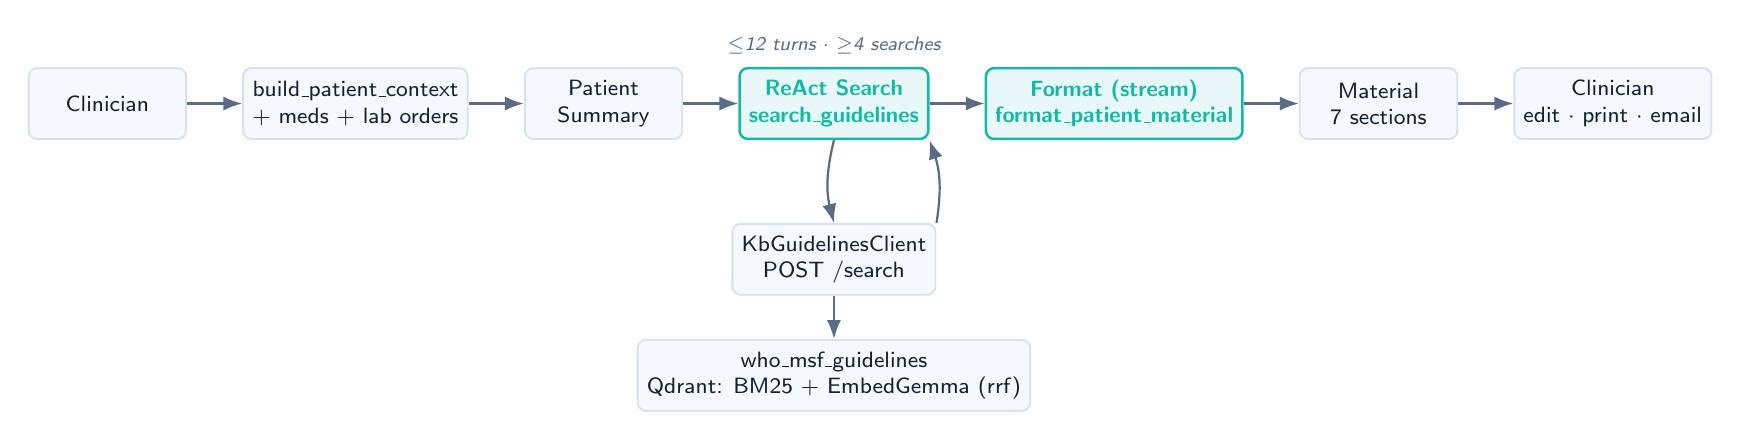
\begin{tikzpicture}[node distance=0.62cm and 0.7cm]
\node[fbox] (clin) {Clinician};
\node[fbox, right=of clin] (ctx) {build\_patient\_context\\+ meds + lab orders};
\node[fbox, right=of ctx] (sum) {Patient\\Summary};
\node[abox, right=of sum] (search) {ReAct Search\\search\_guidelines};
\node[abox, right=of search] (fmt) {Format (stream)\\format\_patient\_material};
\node[fbox, right=of fmt] (mat) {Material\\7 sections};
\node[fbox, right=of mat] (rev) {Clinician\\edit $\cdot$ print $\cdot$ email};
\node[fbox, below=1.05cm of search] (kb) {KbGuidelinesClient\\POST /search};
\node[fbox, below=0.55cm of kb] (idx) {who\_msf\_guidelines\\Qdrant: BM25 + EmbedGemma (rrf)};
\draw[flow] (clin)--(ctx); \draw[flow] (ctx)--(sum); \draw[flow] (sum)--(search);
\draw[flow] (search)--(fmt); \draw[flow] (fmt)--(mat); \draw[flow] (mat)--(rev);
\draw[flow] (search.south) to[bend right=14] (kb.north);
\draw[flow] (kb.north east) to[bend right=14] (search.south east);
\draw[flow] (kb)--(idx);
\node[font=\sffamily\scriptsize\itshape, text=softgray, above=0.04cm of search] {$\leq$12 turns $\cdot$ $\geq$4 searches};
\end{tikzpicture}}

The loop allows a higher budget (\code{MAX\_TURNS = 12}) with the same four-search minimum and the same search-only schema during retrieval. After enough evidence is gathered, Gemma is forced to call \code{format\_patient\_material} (streamed), producing a seven-section document: \emph{What You Have}, \emph{Why It Matters}, \emph{What To Do}, \emph{Your Medications}, \emph{What to Avoid}, \emph{Follow-Up Schedule}, and \emph{When To Seek Help}. The prompt keeps language simple, requires at least four bullets per section, and substitutes ``dose as prescribed by your doctor'' rather than inventing doses; when evidence is missing it defers with ``ask your doctor for specific guidance.'' A \code{\_synthesise\_fallback} provides a safe generic template if the model or KB is unavailable.

The key difference from CDS is the handoff. Patient material is \textbf{editable}: the clinician reviews and adjusts each section inline (\code{editableSections}), optionally translates it, then prints or emails it to the patient. As with CDS, nothing is written back to OpenMRS automatically --- the clinician remains the point of delivery.

\subsection{Plain-Language Reporting}

The report builder is split between model planning and deterministic execution. The model mutates a small \code{ReportSpec}; \code{report\_builder.py} compiles it into a \code{QueryPlan}. The agent never emits raw FHIR URLs. The compiler resolves natural-language date phrases, validates all CIEL concepts locally, chooses filter modes from CIEL datatypes, emits FHIR Observation/Patient/Encounter search descriptors, and defines post-processing such as intersect, union, divide, or group-by.

\diagramfig{Reporting: planning versus deterministic execution}{%
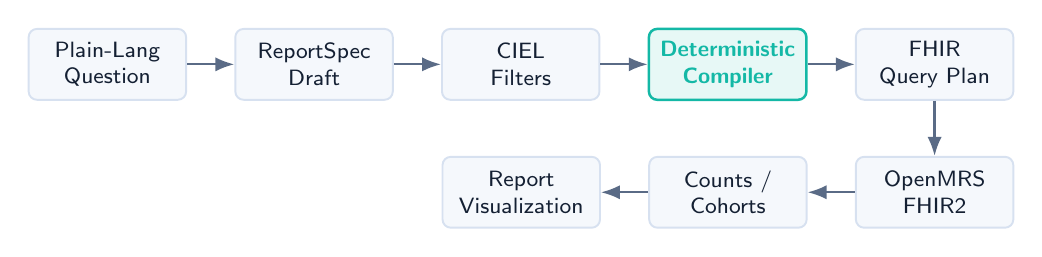
\begin{tikzpicture}[node distance=0.6cm and 0.6cm]
\node[fbox] (q) {Plain-Lang\\Question};
\node[fbox, right=of q] (spec) {ReportSpec\\Draft};
\node[fbox, right=of spec] (ciel) {CIEL\\Filters};
\node[abox, right=of ciel] (comp) {Deterministic\\Compiler};
\node[fbox, right=of comp] (plan) {FHIR\\Query Plan};
\node[fbox, below=0.7cm of plan] (fhir) {OpenMRS\\FHIR2};
\node[fbox, left=of fhir] (res) {Counts /\\Cohorts};
\node[fbox, left=of res] (viz) {Report\\Visualization};
\draw[flow] (q)--(spec); \draw[flow] (spec)--(ciel); \draw[flow] (ciel)--(comp);
\draw[flow] (comp)--(plan); \draw[flow] (plan)--(fhir); \draw[flow] (fhir)--(res); \draw[flow] (res)--(viz);
\end{tikzpicture}}

\code{openmrs\_reader.py} performs the FHIR2 reads and datatype-specific filtering. Boolean observations are filtered client-side by \code{valueBoolean}, coded observations use \code{value-concept} with fallback, and numeric observations are filtered client-side because \code{value-quantity} is unreliable across \OpenMRS{} FHIR2 builds.

% ============================================================ GEPA
\section{GEPA Optimization}

\Product{} uses GEPA as the first adaptation layer because many failures in clinical-informatics agents are instruction and tool-use failures, not missing model weights. GEPA optimizes the prompts that tell Gemma how to search, inspect, reject, and commit concepts. The GEPA-optimized prompts and the high-scoring trajectories they produce then become the supervision for the merged LoRA adapter (Section~8), so the two stages compound: better instructions first, then weights distilled from the behaviour those instructions unlock.

The GEPA runner is offline. \code{run\_form\_gepa.py} configures a task model (local \Gemma{} endpoint), a reflection model (DeepSeek-R1 on Vertex), a dataset of clinician-graded form prompts with \code{requireAnyOf} concept clusters, and a deterministic metric combining CIEL-expanded coverage with schema validity and size constraints.

\begin{safetybox}
\textbf{Train equals serve.} \code{form\_pipeline\_dspy.py} does not build a toy surrogate. It wraps the real \code{run\_form\_pipeline\_agent} and uses \code{prompt\_overlay()} to evaluate candidate prompts inside the actual production pipeline.
\end{safetybox}

\diagramfig{GEPA optimization loop}{%
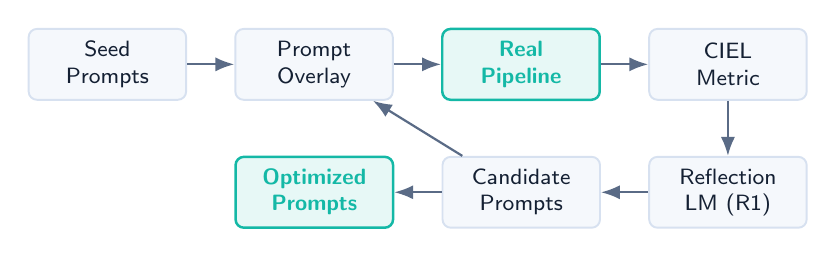
\begin{tikzpicture}[node distance=0.6cm and 0.6cm]
\node[fbox] (seed) {Seed\\Prompts};
\node[fbox, right=of seed] (overlay) {Prompt\\Overlay};
\node[abox, right=of overlay] (pipe) {Real\\Pipeline};
\node[fbox, right=of pipe] (metric) {CIEL\\Metric};
\node[fbox, below=0.7cm of metric] (reflect) {Reflection\\LM (R1)};
\node[fbox, left=of reflect] (cand) {Candidate\\Prompts};
\node[abox, left=of cand] (export) {Optimized\\Prompts};
\draw[flow] (seed)--(overlay); \draw[flow] (overlay)--(pipe); \draw[flow] (pipe)--(metric);
\draw[flow] (metric)--(reflect); \draw[flow] (reflect)--(cand); \draw[flow] (cand)--(overlay);
\draw[flow] (cand)--(export);
\end{tikzpicture}}

Optimized prompts are exported into \code{prompts/optimized/}. Runtime activation is explicit through \code{TENAOS\_USE\_OPTIMIZED\_PROMPTS=1}. Base prompts remain SHA-256 hash pinned, so unintentional prompt drift is caught. The GEPA score is normalized to 0--1; a score of 1.0 means full CIEL-expanded cluster coverage with a valid schema and acceptable field count. The CIEL and report subsets are deliberately small and terminology-hard, so their absolute scores read low; the relevant signal is the \emph{lift} from the seed prompt to GEPA on the real pipeline. The LoRA adapter is reported separately as a training and release artifact; workflow-level LoRA performance claims require a dedicated post-merge evaluation.

\vspace{0.4em}
\begin{center}
\begin{tabular}{>{\raggedright\arraybackslash}p{0.38\linewidth} >{\raggedright\arraybackslash}p{0.18\linewidth} >{\raggedright\arraybackslash}p{0.18\linewidth} >{\raggedright\arraybackslash}p{0.18\linewidth}}
\arrayrulecolor{panebd}\toprule
\rowcolor{brandink}\sffamily\textbf{\textcolor{white}{Metric}} & \sffamily\textbf{\textcolor{white}{Seed}} & \sffamily\textbf{\textcolor{white}{GEPA}} & \sffamily\textbf{\textcolor{white}{Subset}}\\
\midrule
Form CIEL coverage score & 0.118 & 0.246 & CIEL-hard\\
\rowcolor{rowalt}Report coverage score & 0.274 & 0.492 & Report dev\\
Form concept recall & 0.465 & 0.580 & 147 system\\
\rowcolor{rowalt}Schema-valid rate & 0.993 & 0.997 & 147 system\\
Hallucinated/retired-code rate & 3.1\% & 1.2\% & 147 system\\
\bottomrule
\end{tabular}
\\[4pt]
{\footnotesize\color{softgray}Seed = base prompt + base \Gemma{}; GEPA = optimized prompt + base \Gemma{}. These prompt-optimization metrics are not LoRA performance claims.}
\end{center}


% ============================================================ LORA
\section{LoRA Fine-Tuning}

\Product{} ships a \textbf{single task-tagged LoRA adapter} that serves every workflow. Rather than maintaining one model per feature, the adapter is trained multi-task over clinical-informatics behaviours and routed at inference by task tags (\code{[form]}, \code{[report]}, \code{[scribe]}, \code{[scribe-am]}, \code{[cds]}, and \code{[edu]}). The sibling \code{/var/www/LORA\_TenaOS} repository generates, validates, normalizes, and trains the adapter corpus.

The adapter was trained as a BF16 LoRA over the text decoder while the local demonstration runtime remained active. Deployment follows the adapter-merge path: the trained adapter is merged into the BF16 release build, while any quantized deployment artifact is treated as a separate packaging step.

\vspace{0.3em}
\begin{tcbraster}[raster columns=3, raster column skip=7pt, raster row skip=7pt, raster equal height=rows]
  \statcard{16{,}005}{Validated task-tagged traces}
  \statcard{7}{Canonical workflow buckets}
  \statcard{r=16}{LoRA rank ($\alpha$=32)}
\end{tcbraster}

\textbf{Training corpus.} The adapter is trained on a curated, task-tagged SFT corpus. The current SFT split contains 18,909 training conversations, 1,071 validation conversations, and 1,109 held-out test conversations. Records are real multi-turn ShareGPT-style conversations reconstructed from production event traces where available, and training masks loss to assistant turns only.

\textbf{Training-readiness validation.} Every trace teaches assistant-side behaviour --- understanding requests, planning evidence search, searching \WHO{} evidence, selecting \CIEL{} concepts, building artefacts, and marking quality. The validation pass keeps only complete, standards-compatible, training-ready trajectories for adapter training.


\textbf{Training configuration.} The adapter uses \Gemma{} with BF16 LoRA, rank 16, $\alpha$=32, dropout 0.0, attention and MLP adapters, maximum sequence length 24,576, batch size 1 with 8-step gradient accumulation, and 3 epochs over the training split. Runtime was 70.5 hours for 7,086 optimization steps. The final recorded training loss was 0.04123.

\begin{figure}[htbp]
\centering
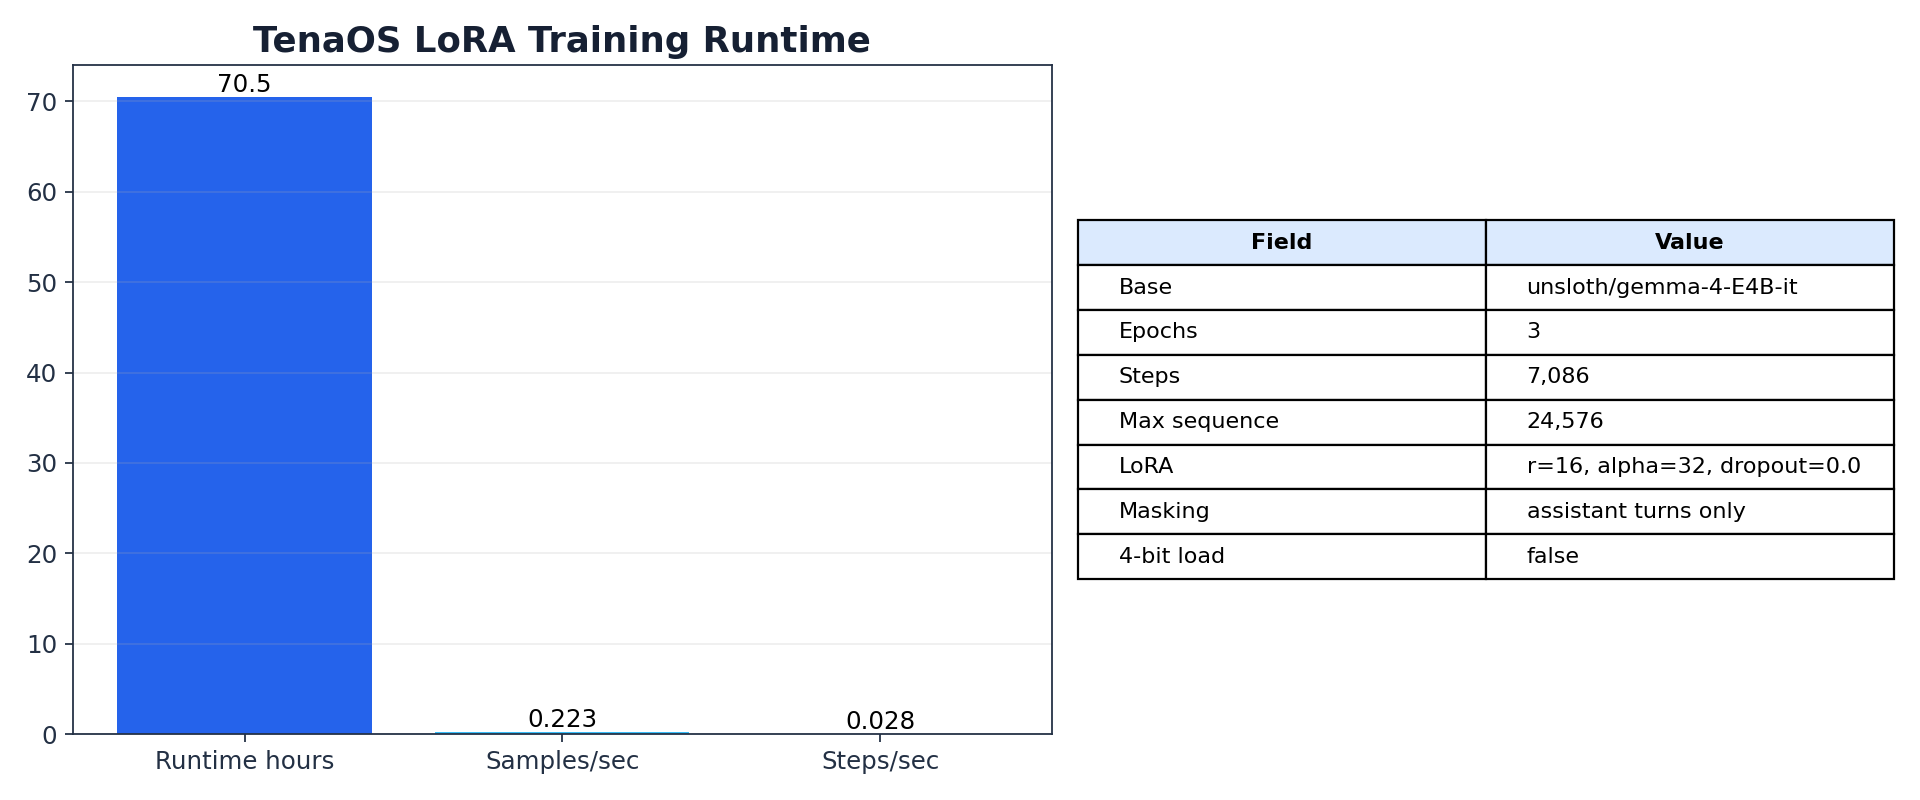
\includegraphics[width=0.96\linewidth]{assets/lora/lora_training_runtime.png}
\caption{Local A100 80GB LoRA training configuration and runtime.}
\end{figure}

\begin{figure}[htbp]
\centering
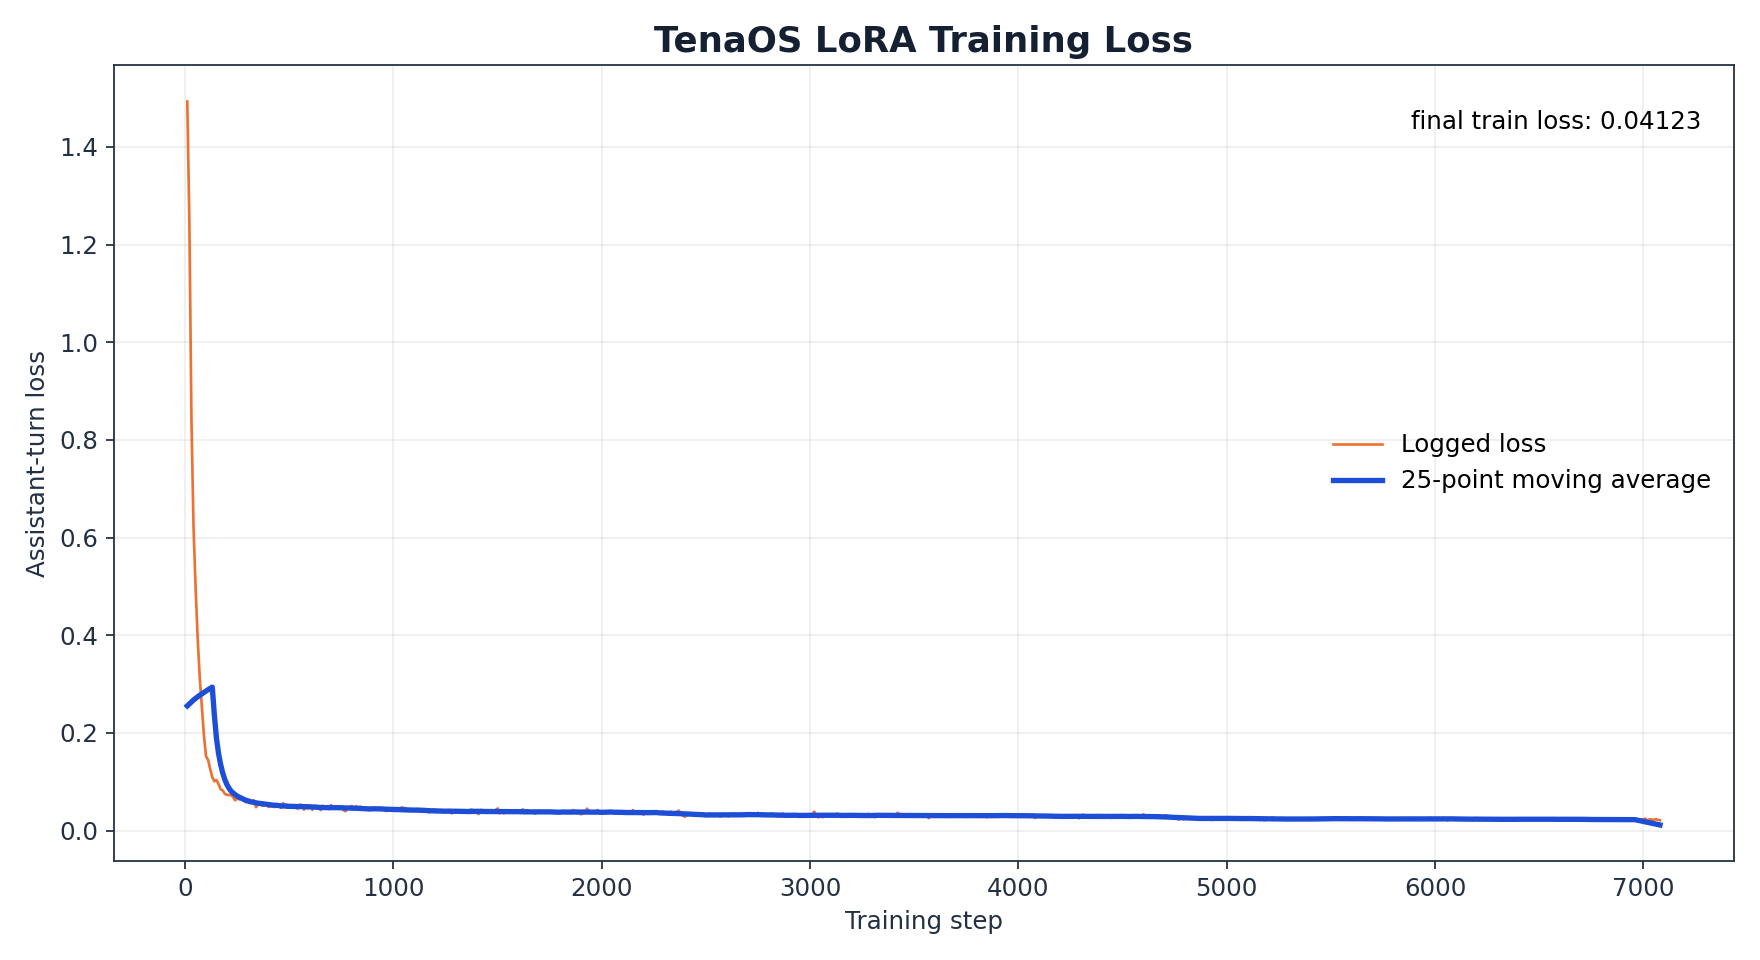
\includegraphics[width=0.96\linewidth]{assets/lora/lora_training_loss.png}
\caption{Training loss over the 3-epoch task-tagged LoRA run. The loss drops rapidly during early adaptation and then stabilizes in a low range.}
\end{figure}

\textbf{Evaluation boundary.} The training curves show that adapter training completed successfully. Workflow-level quality metrics are evaluated separately in the full runtime, preserving the report's separation between model training evidence and clinical-workflow evaluation.


% ============================================================ EVAL
\section{Evaluation Methodology}

The evaluation protocol is detailed in \code{docs/evaluation/evaluation-protocol.md}. The core principle is to separate technical evaluation from clinical validation. The completed technical evaluation package is summarized below.

\vspace{0.4em}
{\footnotesize
\setlength{\LTleft}{0pt plus 1fill}\setlength{\LTright}{0pt plus 1fill}
\setlength{\LTpre}{0pt}\setlength{\LTpost}{0pt}
\begin{longtable}{>{\raggedright\arraybackslash}p{0.18\linewidth} >{\raggedright\arraybackslash}p{0.40\linewidth} >{\raggedright\arraybackslash}p{0.32\linewidth}}
\arrayrulecolor{panebd}\toprule
\rowcolor{brandink}\sffamily\textbf{\textcolor{white}{Workflow}} & \sffamily\textbf{\textcolor{white}{Key metrics}} & \sffamily\textbf{\textcolor{white}{Completed evidence}}\\
\midrule
\endfirsthead
\arrayrulecolor{panebd}\toprule
\rowcolor{brandink}\sffamily\textbf{\textcolor{white}{Workflow}} & \sffamily\textbf{\textcolor{white}{Key metrics}} & \sffamily\textbf{\textcolor{white}{Completed evidence}}\\
\midrule
\endhead
\bottomrule
\endlastfoot
Form builder \& GEPA & CIEL-expanded recall, exact recall, schema-valid rate, hallucinated/retired-code rate, tool calls, latency, publish readiness & GEPA prompt-optimization package complete; LoRA workflow evaluation remains separate\\
\rowcolor{rowalt}WHO/MSF retrieval & Retrieval scale, local indexing, hybrid retrieval, reranker design, citation grounding & 69,476 chunks (EmbedGemma + BM25); 448.8\,MB Qdrant snapshot\\
CIEL retrieval \& validation & Concept/mapping coverage, retired handling, bundle hydration, concept identity & 58,687 concepts, 298,905 mappings, 8,545 Q\&A edges, 3,259 set edges\\
\rowcolor{rowalt}Scribe & SOAP completeness, concept F1, medication structuring, ASR WER, unresolved handling & Text, voice, and Amharic trace corpus included in LoRA training; workflow extraction and WER evaluation remain separate\\
Report builder & Query-plan correctness, count accuracy, datatype filter-mode, compile success & Deterministic compiler implemented with Boolean, coded, numeric, condition, and any-value filter modes\\
\rowcolor{rowalt}CDS \& patient education & Citation grounding, unsupported-rec rate, abstention correctness, dose safety, clinician review & Agentic guideline search and cited-output workflows implemented over the local WHO/MSF KB; full workflow evaluation remains separate\\
Deployment & Local footprint, model serving, Qdrant restore, single-container operation & Single-container runtime; Gemma GGUF + mmproj + LoRA; Q4/BF16 tiers; 448.8\,MB + 326.3\,MB snapshots\\
\end{longtable}
}

% ============================================================ SAFETY
\section{Responsible AI and Safety}

\Product{} is built around layered controls:

\begin{itemize}
  \item \textbf{Local data boundary:} \OpenMRS{}, model inference, \CIEL{}, Qdrant, and trace stores run locally.
  \item \textbf{Allow-listed tools:} Gemma uses only exposed, allow-listed tools.
  \item \textbf{Retrieval grounding:} CDS and patient education use retrieved \WHO{} evidence.
  \item \textbf{Terminology validation:} final clinical records use \CIEL{} bundles and \OpenMRS{} concept IDs.
  \item \textbf{Deterministic middleware:} schema builds, report plans, concept filters, and \OpenMRS{} writes are compiled and checked outside the model.
  \item \textbf{Human review:} forms, scribe outputs, patient materials, and recommendations are reviewable before use.
  \item \textbf{Audit traces:} workflows persist or stream tool calls, retrieval results, and draft evolution.
\end{itemize}

The system card in \code{docs/system-card.md} documents intended use, users, outputs, contraindicated uses, risks, mitigations, and monitoring.

% ============================================================ GOVERNANCE
\Needspace*{12\baselineskip}
\section{Clinical Governance Boundary}

\begin{safetybox}
\textbf{Governance invariant.} \Product{} produces evidence-grounded, standards-based drafts that pass through deterministic validation and clinician review before clinical persistence. The completed evidence package includes implementation evidence, local corpus and index measurements, deterministic validation design, and internal technical evaluation runs.
\end{safetybox}

% ============================================================ REPRO
\section{Reproducibility}

Important entry points:
\begin{itemize}
  \item Runtime setup: \code{README.md}, \code{scripts/setup-demo.sh}, \code{scripts/fetch-models.sh}.
  \item Agent workflows: \code{TenaAgent/README.md}, \code{TenaAgent/service/tena\_agent\_service/}.
  \item \WHO{} KB runtime: \code{TenaOS-KnowledgeBase/}; build: \code{kb-pipeline/} build tree.
  \item \CIEL{} build/runtime: \code{TenaOS-CIEL/}.
  \item GEPA optimization: \code{scripts/optimization/}.
  \item LoRA corpus and adapter training: \code{/var/www/LORA\_TenaOS}.
\end{itemize}

% ============================================================ TECHNOLOGIES
\Needspace*{16\baselineskip}
\section{Technologies Used}

\begin{itemize}
  \item \textbf{OpenMRS} --- open-source medical record system.
  \item \textbf{CIEL} --- Columbia International eHealth Laboratory concept dictionary.
  \item \textbf{FHIR R4} --- reporting read interface through \OpenMRS{} FHIR2.
  \item \textbf{WHO and MSF clinical guidance} --- local guideline evidence corpus.
  \item \textbf{Gemma 4 E4B} --- local multimodal generation model (text, voice, image).
  \item \textbf{LoRA / PEFT} --- single task-tagged adapter fine-tuned on validated \Product{} traces.
  \item \textbf{EmbedGemma 300M} --- dense retrieval model for guideline chunks.
  \item \textbf{SapBERT} --- dense biomedical concept encoder for \CIEL{} semantic search.
  \item \textbf{Qdrant} --- local vector database for dense and sparse retrieval.
  \item \textbf{GEPA/DSPy} --- offline prompt optimization framework.
\end{itemize}

\end{document}
